\documentclass[sigconf]{acmart}

\usepackage{booktabs} % For formal tables

\usepackage{url}
%Workgroup Lutteroth&Weber defs
%general language defs
\usepackage{xspace}
\newcommand{\eg}{e.g.,\ }
\newcommand{\ie}{i.e.,\ }
%command to add TODOs in the document so that they can be switched on/off centrally
%The command that shows the TODO in the printout. Uncomment that as long as the document is in preparation.
\newcommand{\todo}[1]{\textbf{\{TODO: #1\}}}                 
%The command that hides the TODO. Uncomment that for submission
%\newcommand{\todo}[1]{}     
\DeclareMathOperator*{\argmin}{arg\,min}

% Copyright
%\setcopyright{none}
%\setcopyright{acmcopyright}
%\setcopyright{acmlicensed}
% 

%\setcopyright{usgov}
%\setcopyright{usgovmixed}
%\setcopyright{cagov}
%\setcopyright{cagovmixed}


% DOI
% \acmDOI{10.475/123_4}  

% % ISBN
% \acmISBN{123-4567-24-567/08/06}

% %Conference
% \acmConference[WOODSTOCK'97]{ACM Woodstock conference}{July 1997}{El
%   Paso, Texas USA}
% \acmYear{1997}
% \copyrightyear{2016}


% \acmArticle{4}
% \acmPrice{15.00}
 
% These commands are optional
%\acmBooktitle{Transactions of the ACM Woodstock conference}
% \editor{Jennifer B. Sartor}
% \editor{Theo D'Hondt}
% \editor{Wolfgang De Meuter}

 
\begin{document}
\title{SwiftLaTeX- Exploring Web-based %the potentials of 
True WYSIWYG Editing for Digital Publishing}
%\titlenote{Produces the permission block, and  copyright information}
 

\author{Elliott Wen}
% \orcid{1234-5678-9012}
\affiliation{%
  \institution{The University of Auckland}
}
\email{jq.elliott.wen@gmail.com}

\author{Gerald Weber}
\affiliation{%
  \institution{The University of Auckland}
}
\email{g.weber@auckland.ac.nz}

\copyrightyear{2018} 
\acmYear{2018} 
\setcopyright{acmlicensed}
\acmConference[DocEng '18]{ACM Symposium on Document Engineering 2018}{August 28--31, 2018}{Halifax, NS, Canada}
\acmBooktitle{DocEng '18: ACM Symposium on Document Engineering 2018, August 28--31, 2018, Halifax, NS, Canada}
\acmPrice{15.00}
\acmDOI{10.1145/3209280.3209522}
\acmISBN{978-1-4503-5769-2/18/08}

% The default list of authors is too long for headers.
%\renewcommand{\shortauthors}{B. Trovato et al.}


\begin{abstract}
The text processing tool \LaTeX\ has prevailed as a standard in many fields of exact sciences; it is evident that  \LaTeX\ is likely to be here to stay. 
From that perspective, it is important to explore what are the best possible ways to support the author in efficiently editing documents. There have been several approaches that provide graphical editing support for \LaTeX. 
We argue that a true WYSIWYG (What You See Is What You Get) approach is a justified requirement for future systems and we present here the first cloud-based true WYSIWYG editor. This allows the author to edit the document in its print form directly in a web-based PDF viewer. 
Building such a system creates unique challenges compared to existing approaches. 
We identify these challenges and name workable solutions. 
We also provide a usability evaluation of the new system. 
%!!!
In short our finding is that editing \LaTeX\ directly in the PDF view is possible for a wide range of edits and valuable for many major user groups and use cases; hence it is a fair requirement for future top-of-the-line \LaTeX\ editors. \end{abstract}

%
% The code below should be generated by the tool at
% http://dl.acm.org/ccs.cfm
% Please copy and paste the code instead of the example below.
%
\begin{CCSXML}
<ccs2012>
<concept>
<concept_id>10003120.10003121.10003124.10010865</concept_id>
<concept_desc>Human-centered computing~Graphical user interfaces</concept_desc>
<concept_significance>500</concept_significance>
</concept>
<concept>
<concept_id>10003120.10003121.10003128.10011753</concept_id>
<concept_desc>Human-centered computing~Text input</concept_desc>
<concept_significance>500</concept_significance>
</concept>
</ccs2012>
\end{CCSXML}

\ccsdesc[500]{Human-centered computing~Graphical user interfaces}
\ccsdesc[500]{Human-centered computing~Text input}

% \keywords{ACM proceedings, \LaTeX, text tagging}


\maketitle
%%%%%%%%%%%%%%%%%%%%%%%%%%%%%%


%body
\section{Introduction}  

The \TeX\ typesetting system developed by Donald Knuth ushered in an era of high-quality open-source electronic document publishing. 
Knuth embedded  deep knowledge of the traditional art and craft of typesetting into \TeX\. 
%As a result, \TeX\ produces print-ready documents that adhere to the highest standards of print aesthetics.  
Over the intervening decades, various \TeX\ derivatives have established themselves. 
Among them, \LaTeX\ is particularly widespread and maintained by a large community.

%automatically handles the low-level typesetting and encourages users to focus on content editing.
% \LaTeX\ i  

% provides a higher-level language that accesses the power of TeX in an easier way for writers.
%   provide a high-level language that accesses the power of TeX in 

However, the \TeX\ family of tools exhibits a major usability limitation due to their nature as batch processing systems which results in an edit-compile-review cycle. 
This cycle is generally acknowledged to possess certain usability disadvantages; 
the user is forced to perform difficult mental mappings back and forth between the one-dimensional textual \TeX\ source codes and the two-dimensional graphical print output, displayed on the screen only after a slow compilation process \cite{brown2013integrated}. This takes longer than the time which users are known to find acceptable in interactive systems. It renders various editing tasks fairly inefficient such as proofreading, which often involves a large share of single-character edits.

% which can be summarized in the statement that LaTeX is classically understood to require programming-like skills.
A number of partial solutions to  this problem have been developed. 
Some \LaTeX\ editors (e.g., ShareLatex \cite{oswaldsharelatex}, now merged with Overleaf \cite{overleaf}) provide asynchronous and regular refresh of the print output, which is placed side by side with the code editor. 
Optionally, the editor also features formatted text input, %(often referred to as WYSIWYM, \ldots What You \textit{Mean}) 
where a fixed number of \LaTeX\ text style commands 
are displayed in different colors and fonts accordingly, \eg section headers are shown in a large and bold font.
However in these approaches there is still a large discrepancy between the edit view and the print layout view and the user has to alternate and switch focus between them in many work cycles. 

%\todo{bad transition? probably: works actually without transition.}
%Nevertheless, these works still shed light to us. 
A thorough analysis of these existing solutions (see Section~\ref{sect:background}) leads us to the research hypothesis that enabling WYSIWYG editing of  \LaTeX\ documents directly in the print (PDF) layout will bring about a significant improvement in usability for various user groups due to the removal of the notorious edit-compile-review cycle. 
To match this aspiration, and to keep the usability advantages gained with current cloud services, we introduce SwiftLaTeX, the first cloud-based \LaTeX\ true WYSIWYG system for.


However, implementing a responsive WYSIWYG editor entails three challenges. First, allowing direct editing of the PDF document requires that the product of the \LaTeX\ compilation must be combined with the new user input as quickly as possible. This is challenging since traditional recompiling is too slow for character-wise quick response.
Secondly, the editor is expected to intercept the modification on the PDF document and to  apply the alternation synchronously in the corresponding position of the source code.  
To achieve this, the editor requires the ability to infer the source code position of each element in the PDF with character-wise accuracy. 
This is a stretch target since the highest level of accuracy in  existing open-source tools is merely line-level.
Finally, for a cloud-based system with a massive number of potential users, maintaining high scalability, reliability and compatibility remains a challenging issue, 
%new:
particularly since as long as we rely on repeated compilations, there is an obvious  tradeoff between computing resource consumption and responsiveness.

In this paper, we present practical solutions to cope with the above challenges. Specifically, to correctly combine the product of the \LaTeX\ compilation and the user's editing, SwiftLaTeX proposes an asynchronous merging mechanism.
To infer the source code positions, SwiftLaTeX explores an advanced text-matching algorithm and dynamically patches the \LaTeX\ engine with a bookkeeping mechanism in pursuit of character-level accuracy. To achieve high scalability, reliability and compatibility, SwiftLaTeX embraces a distributed system back-end architecture and features a responsive front-end design. 

We consolidated the above techniques and implemented a  prototype of SwiftLaTeX on cloud computing platforms, based on which we conducted a preliminary user study involving six \LaTeX\ users to evaluate the usability aspects of the system. The evaluation results show that participants reacted positively to the innovative web-based editable PDF viewer and praised its efficiency for certain editing tasks such as proofreading.

To sum up, the main contributions of this paper are as follows.
\begin{enumerate}
\item We provide a review of existing \LaTeX\ editors in Section~\ref{sect:background} and derive requirements for our system as a cloud-based WYSIWYG editor in a narrower sense in Section~\ref{sect:usability}.
\item We propose a high-level algorithmic standard architecture for asynchronous WYSIWYG editors working on a batch-style text processing system in Section~\ref{sect:challenges}.
\item We implement and integrate a fine-grained source code positioning system in \LaTeX\ system in Section~\ref{sect:textpos}.
\item We present a working cloud-based prototype which is scalable, reliable and compatible with mainstream browsers on different kinds of devices in Section~\ref{sect:imp}. 
\item We conduct a preliminary pilot study evaluating usability aspects of the system in Section~\ref{sect:eve}.
\end{enumerate}




% We explain how our system succesfully fulfils this criterion. 

% Specifically, SwiftLaTeX provides the authentic WYSIWYG editing experience for \LaTeX\ users by transforming a passive viewer to an editable one. 
% Such a move brings about significant benefits for various user groups.

% make the first attempt at direct editing in the print output, which is a natural solution to avoid the notorious edit-compile-review cycle. 
% The move from a passive viewer to an editable view is one of the few classic user interface evolutions 
% where it is hard to argue that it is not an improvement of usability. 
% The only question is usually how complete the edit features are.
% Nevertheless, these works still shed light on us and 
% One natural solution to avoid the edit-compile-review cycle 
% a systematic discussion of them from the usability aspects (see Section~\ref{sect:background}) reveals a key insight that direct editing in the print output will be a natural solution to avoid the edit-compile-review cycle and beneficial for many user groups in certain tasks.

% motivates us to explore a novel approach that enables direct editing in the PDF view. 
% In this work, we introduce SwiftLaTeX, a novel system that explores true WYSIWYG editing for digital publishing.
% Nevertheless, these works still shed light to us. A systematic discussion of them from the usability aspects (see Section~\ref{sect:usability}) motivates us to explore a novel approach that enables direct editing in the PDF view. 
% Nevertheless, these works still shed light to us and a systematic discussion of them from the usability aspects motivate us.
% % In Section~\ref{sect:usability} we give a systematic discussion of these and further usability aspects  of such editors. 
% A main purpose of this section is to establish that direct editing in the PDF view is clearly useful for many user groups at least for some tasks.
% The move from a passive viewer to an editable view is one of the few classic user interface evolutions 
% where it is hard to argue that it is not an improvement of usability. The only question is usually how complete the edit features are.


% The aim of this article is in short to present our current findings in search for an editor to match these aspirations. 
% We present our demonstration system that is a web-based editable PDF viewer for LaTeX. 
% We define an important basic completeness criterion for the capabilities of a print-quality WYSIWYG editor, the replacement capability:  All text that is visible in the resulting PDF document, including basic text in formulae for instance, is editable resp. replaceable, \ie we can exchange $\frac{4}{cx}$ against $\frac{4}{ct}$ visually and instantaneously. 
% We explain how our system succesfully fulfils this criterion. 
% We categorize the natural limitations of the approach, for example with regard to structural changes. 


\section{Background of the \LaTeX\ family of systems}\label{sect:background}

\subsection{Factors influencing the future of the  \TeX\ family}
Donald Knuth's program \TeX\ is one of the  few notable programs developed back in the 1970s that are still in use today. 
%Even almost fifty years after its inception, the program is still used intensively, mostly via its renowned derivative named \LaTeX.
There are several factors that make the continued use and significance of \TeX\  and its derivative  \LaTeX\  very plausible in the foreseeable future: 

{\bf Excellent Output Quality:} \LaTeX\,  with its built-in typesetting expertise,  manages to generate output considered by many to be unsurpassed in quality.

{\bf Technical Stability:} The stability of \LaTeX\ has been proven by its intensive use by millions of users with demanding input.

{\bf Format Stability:} Since the minor switch to \LaTeX\ 2e in 1994, the central component of the \LaTeX\ engine has not undergone any incompatible version changes, which ensures that old source packages continue to work. 

{\bf Strong Maintenance Support from Community:}  A large and stable community is maintaining the system in a self-organized fashion, which is nurturing the technical innovation for \LaTeX.

{\bf Community Investment:}  Many communities using \LaTeX\ are heavily invested in it in the sense that many of the workflows and assets in the shape of \LaTeX\ stylesheets are locked-in to \LaTeX.


\subsection{Systematics of \LaTeX\ Editing Systems}
Over the past decade, various editing systems have been developed to make \LaTeX\  editing more convenient.  
% The aforementioned issues are negatively affecting a number of \LaTeX\ editing systems, 
They can mainly be divided into two categories, standalone versus web-based, or cloud-based.

\textbf{Standalone:} 
The most rudimentary standalone systems are command line based applications  (e.g., {Latexmk} \cite{collins2015latexmk} and {LatexRun} \cite{latexrun}), which commonly serve as automated compilation tools. 
Given a set of source files, these tools issue the appropriate sequence of commands to communicate with the typesetting engines and generate the resulting document. 
Generally, the command line programs are rarely invoked directly due to debugging difficulty. 
Instead, they  are commonly utilized as the backend for the graphical editors.

\textbf{Integrated Development Environments (IDEs):}
Graphical editor applications (e.g., TeXstudio \cite{vantexstudio}, TeXworks, TeXnicCenter and TeXshop \cite{koch2006texshop}) aim to facilitate document editing by providing a graphical user interface (GUI) with various features such as syntax highlighting and automated error correction. 
These features significantly reduce the difficulty of debugging and increase the editing productivity.
% Despite the promising features, these IDEs still suffer from the notorious edit-compile-review cycle.
Nevertheless, setting up such an editor may involve difficult and laborious configurations (e.g., installing \LaTeX\ packages and maintaining software dependency), which is not user-friendly for novice users. 
This gap opens opportunities for the emergence of web-based editing systems.

\textbf{Desktop WYSIWYG editors:}
Desktop WYSIWYG editors work in a very similar way to office tools: The open-source tool LyX \cite{kastrup2002revisiting} acknowledges that the edit view does not reflect the print output and calls the approach WYSIWYM (what you see is what you Mean).
The Bakoma \TeX\ tool~\cite{soft2011bakoma} is a WYSIWYG editor in the narrower sense. 

\textbf{Web-based editors:}
Compared with the standalone editors, the web-based editing systems possess a distinct advantage, namely zero set-up time. 
Specifically, these web-based editing systems run instantly on at least some mainstream browsers and require no software installation on the users' devices. 
In other words, web-based systems make \LaTeX\ rapidly and easily accessible in the user's web browsers.
Another merit of the web-based system is cloud storage, which enables project files to be accessed anywhere in the world and greatly facilitates collaboration. 
These advantages make web-based systems fairly prominent; the most popular platform, Overleaf now  has over 6 million users and hosts over 10 million projects \cite{overleafstat}. 
It is therefore not far-fetched to assume continuing growth of web-based \LaTeX\ editing and argue that any innovation on web-based, cloud-based \LaTeX\ editing systems is making a substantial contribution to digital publishing in the 21st century.

\subsection{Limitations of Current Editing Systems}
However, despite the invaluable features of the \TeX\ family, they possess major limitations, namely a steep learning curve, and the batch-style text processing as well as the lack of structure in LaTeX scripts.
Specifically, it is generally accepted that the script language of \LaTeX\  poses a substantial technical hurdle for novice users \cite{gratzer2008gentle}. 
The batch processing nature  further aggravates this problem; the necessary edit-compile-review cycle  is generally acknowledged to possess certain usability disadvantages.
First, it further steepens the learning curve for  beginners who have to wait for the time-consuming compilation process to finish before they can examine whether the resulting document is correct. 
If not, they have to go back to the editor and pinpoint which line of the source code is causing the problem. 
The demanding debugging-like process tends to cause a sense of confusion and frustration. 
More importantly, users are now forced to carry out intensive mental mappings back and forth between the essentially one-dimensional textual \TeX\ source codes and the two-dimensional graphical print output \cite{brown2013integrated}. 
It can make certain editing tasks such as single-character edits very inefficient. 

% Recently, the cloud-based editing systems such as ShareLatex \cite{oswaldsharelatex} and Overleaf \cite{overleaf} are becoming fairly prominent due to their distinguishing advantages, namely, zero set-up time, simple collaboration, and enhanced user interfaces.
% Specifically, these cloud-based editing systems run instantly on any mainstream browsers. In other words, no software installation is ever required on users' devices. 
% Meanwhile, the users' projected files are stored in the cloud and can be easily accessed anywhere in the world. 
% It thus greatly facilitates  collaboration.

A number of partial solutions have been developed to solve this problem. The most widely-used one utilized by web-based systems is to provide asynchronous and regular refresh of the resulting document, which is placed side by side with the code editor. 
The editor in Overleaf is referred to as the 'Rich Text' feature, where the source code is styled in different colors and fonts accordingly to the categories of terms. 
Still, there exists a strong visual disagreement between the source and compiled document and the user has to alternate and switch focus between them in many cases.

Accordingly we aim to take the term WYSIWYG literally, which naturally raises the research question: how much improvement of usability would true WYSIWYG (i.e., enabling direct editing in the print form) bring about due to the removal of the edit-compile-review cycle. 
We will first clarify the definition of the term in a narrower sense in Section~\ref{sect:usability}.
We then present our research findings during the implementation of SwiftLaTeX, which is the first web-based, cloud-based WYSIWYG \LaTeX\ editing system. 
We report the  challenges we encountered and provide the corresponding open-source solutions.



% To further address this problem, Overleaf is exploring a novel approach advertised as `WYSIWYG' editing. In brief, the editor now features formatted source code inputs, where a fixed number of \LaTeX\ text style commands are displayed
% The `WYSIWYG' paradigm is also advertised by several standalone open-source editors (e.g., LyX \cite{kastrup2002revisiting} and the commercial Bakoma Tex \cite{soft2011bakoma}), which however provide different usability experience.
% We will a narrow definition of the term `WYSIWYG' in the next section.


% In details, the interfaces are enhanced in two aspects. First, the complication process is carried out asynchronously to provide regular refresh of the print output.
% Second, the editors feature an optional rich-text view, where a fixed number of \LaTeX\ text style commands are displayed in different colors and fonts accordingly. 


% Most GUIs consist of two components including a source code editor and a document viewer. 
% The editor usually features syntax highlighting and automatically pinpoints errors if detected.
% The viewer automatically reloads the latest document whenever the a complication process is finished.


\section{Usability Requirements Analysis for a WYSIWYG editor} \label{sect:usability}
The core usability question that we are focusing on in this work is the notion of a WYSIWYG editor. 
The term is often used in a loose manner. However there seems widespread consensus that "Rich Text" views, as for example used currently in Overleaf, should be kept in a separate category. 
In this section, we provide a usability requirement analysis of WYSIWYG editing for \LaTeX\ in a narrower sense.
Note that since we focus on this question here, we consider here other important usability questions such as collaboration/project management to be out of scope.
 
\subsection{WYSIWYG in the narrower sense} \label{sect:wysiwyg}
For the following discussions we introduce an important definition, the notion of \emph{editing quiescence}. 
Editing quiescence is a point in time during use of the editor when the editor has processed all previous edits of the user, and there are hence no pending edits that would further change the output. 
With this definition we can in turn provide the following definition:
A WYSIWYG editor in the narrower sense is an editor fulfilling the following requirements: 
\begin{enumerate}
\item At editing quiescence, the editor shows the print layout of the document, i.e., acts as a faithful print viewer. 
\item At editing quiescence, the user can position the cursor anywhere in the document with the mouse, arrow keys or a combination thereof.
\item The user can perform edits at the cursor position by simply typing the keys or backspace and get immediate feedback in the sense that the editor shows a \textit{preview version} of the print view. 
\item If the user input pauses, the editor reaches editing quiescence automatically in a reasonable amount of time (which can, however, be as long as a \LaTeX\ compile cycle). 
\end{enumerate}

Requirement 4 together with 1 means that the editor replaces the possible preview version with the faithful print view.
The requirement 1 is the one characterizing WYSIWYG in the narrower sense; we argue that this is the actual literal translation of the acronym.
A surprising fact is that the editor created in this project is apparently one of the few cloud-based WYSIWYG editors that is available at all in the narrower sense, not only in the \LaTeX\ domain.
Requirement 3 is asking for the following replacement capability: all text that is visible in the resulting PDF document (including the basic text in formulae) is editable.  For instance, a formula $\frac{4}{cx}$ in the PDF document can be modified to $\frac{4}{ct}$ instantaneously and in place in the PDF. 

In contrast, many WYSIWYG editors that are part of office suites do not fully meet Requirement 1. 
They offer faithful print views only in a non-editable form and rather offer editable WYSIWYG views in a weaker sense: 
The editable view might represent all text styles, including font changes and tabulation, but the edit view is notably different from the print view and can include incorrect word wraps or even page breaks. 
The community of the system LyX makes the case that this can also be seen as a feature and has introduced the term WYSIWYM (what you see is what you mean) to characterize such an editor.
We argue that there is a clear need for WYSIWYG editing: It is commonly acknowledged that in particular final edits in a close-to-print document take a disproportionate amount of time in a non-WYSIWYG editor due  to the turnaround between edit view and print view.   The Bakoma \TeX\ system offers WYSIWYG for a non-cloud based setting.

An even weaker form of a formatted editor should not be included in the WYSIWYG paradigm and instead should be referred to as Rich Text View. 
In a rich text view for \LaTeX\  only a fixed number of text style commands are translated into formatted representation. 
The classically used text styles include headers, bold, italic, typewriter, bullet-lists and enumerations. 
In a \LaTeX\ rich text viewer, only the commands corresponding to these features are hidden and the editable text is formatted accordingly. 
The difference from a weak WYSIWYG editor is that the formatted representation does not change with stylesheet changes, \ie if a different font family is chosen, or a subsection is rendered with small-caps. 
In a classic rich text view, subsections are always rendered with the same header style.


%
%\subsection{Personae and Use Cases} \label{sect:person}
%The WYSIWYG in the narrower sense is useful for many major user groups in a wide range of editing tasks in digital publishing.
%There is certainly still room for a more detailed analysis of all the different personae and use cases for \LaTeX\, but in all detail this would go beyond the scope of this project. We therefore focus on two essential use cases on a standard route to publication, which represent the earliest and latest phase, namely initial writeup and proofreading correction.
%
%At the initial writeup stage, SwiftLaTeX can significantly benefit users, particular novice ones, who wish to focus on content composition and simultaneous learning of \LaTeX. For instance, a scholar can begin to write a thesis using the WYSIWYG editor while having no any \LaTeX\ skills at all. Nevertheless, he can gradually accumulate the knowledge of \LaTeX\ by occasionally peeking at the \LaTeX\ source files automatically generated by SwiftLaTeX. 
%
%At the proofreading stage, the persona to get into contact with a document would be often a language proofreader.
%The edits that they perform are typically very minor on the level of single letter changes.
%Still they would have to go to the source code and pinpoint the corresponding positions for the characters to be modified in conventional \LaTeX\ editors. 
%Such a process tends to repeat quite often, leading to the low efficiency of proofreading.
%SwiftLaTeX overcomes this issue by enabling the proofreaders to directly modify any visible characters on the PDF view without examining the \LaTeX\ source codes. 
%It alleviates the technical hurdle and boosts the efficiency for a proofreader to work on a \LaTeX\ document.
%
%There are certainly personae who would benefit less from a WYSIWYG approach or can simply not use a WYSIWYG editor for certain tasks, for example \LaTeX\ users who make heavy use of custom \LaTeX\ commands. A key question for future work will be whether such users can be enticed to use the WYSIWYG approach for a considerable fraction of their time.
%

%%%%%%%%%%%%%%%%%%%%%%%%%%%%%%%%%%%
% A typical process of analyzing usability questions is to create personas and use cases. 
% Personas are narrative representations of all important user groups of a system. Use cases are tasks that users have to preform. 
% Personas can share use cases but there can be noticeable differences how different personas perform the same use case.
% \todo{we need to illustrate the use cases}
% To start with important use cases, it is useful to distinguish: initial writeup, amendment, correction and proofreading, the latter both technical and for spelling/grammar/style.

% To give a simple example, one of the last persona to get into contact with a document would be often a language proofreader. The edits that they perform are often very minor on the level of single letter changes typically. Yet proofreaders are sometimes not proficient with LaTeX. 
% %\subsection{Personae and tasks of Authors} \ref{sect:person}



\section{Challenges in Asynchronous Compilation for a WYSIWYG editor} \label{sect:challenges}

The aim of allowing direct editing of the PDF document creates completely novel system challenges not faced in current asynchronous cloud-based systems, namely that the product of the \LaTeX\ compilation process must be combined with the current user edit. 


SwiftLaTeX offers two different editing views. The first one is the source view. 
This is inherited from the conventional cloud-based systems, which allow advanced users to directly manipulate \LaTeX\ source code in a classical ASCII editor and to preview the PDF on a separate viewer. 
The source view needs to be preserved because only in source code can arbitrary \LaTeX\ scripting be done.  %(e.g., changing the document template or adjusting the page margin)  can be more conveniently altered in the source code. 

Nevertheless, the main contribution of SwiftLaTeX is the second view, the WYSIWYG view.
This is an editable PDF viewer that allows the user to directly edit a document in its print form, but with effect on the source.
% built on top of the HTML5 and Javascript technologies. Briefly speaking, the viewer is able to render a PDF on the screen with a set of HTML5 elements.
To start an edit, the user simply clicks on any visible text that should be modified. 
A text cursor will appear indicating that the viewer is now ready for the user's input as shown in Fig~\ref{fig:editingexample} (a).
Afterwards, all editing operations such as character appending or removal will instantly be  rendered on the viewer.
%The viewer offers the user with an immediate impression of what the modified document will look like, in other words, a \textit{preview version} of the  PDF.
As mentioned in the requirement 3 in Section \ref{sect:usability},  the instant rendering is a \textit{preview version} of the PDF.
Meanwhile, to retain the modification, the user's editing operations will also be applied at the corresponding position of the \LaTeX\ source code. After the re-compilation process, the user will automatically be presented with the new \textit{revised version} of PDF. 

\begin{figure}[t]
\begin{center}
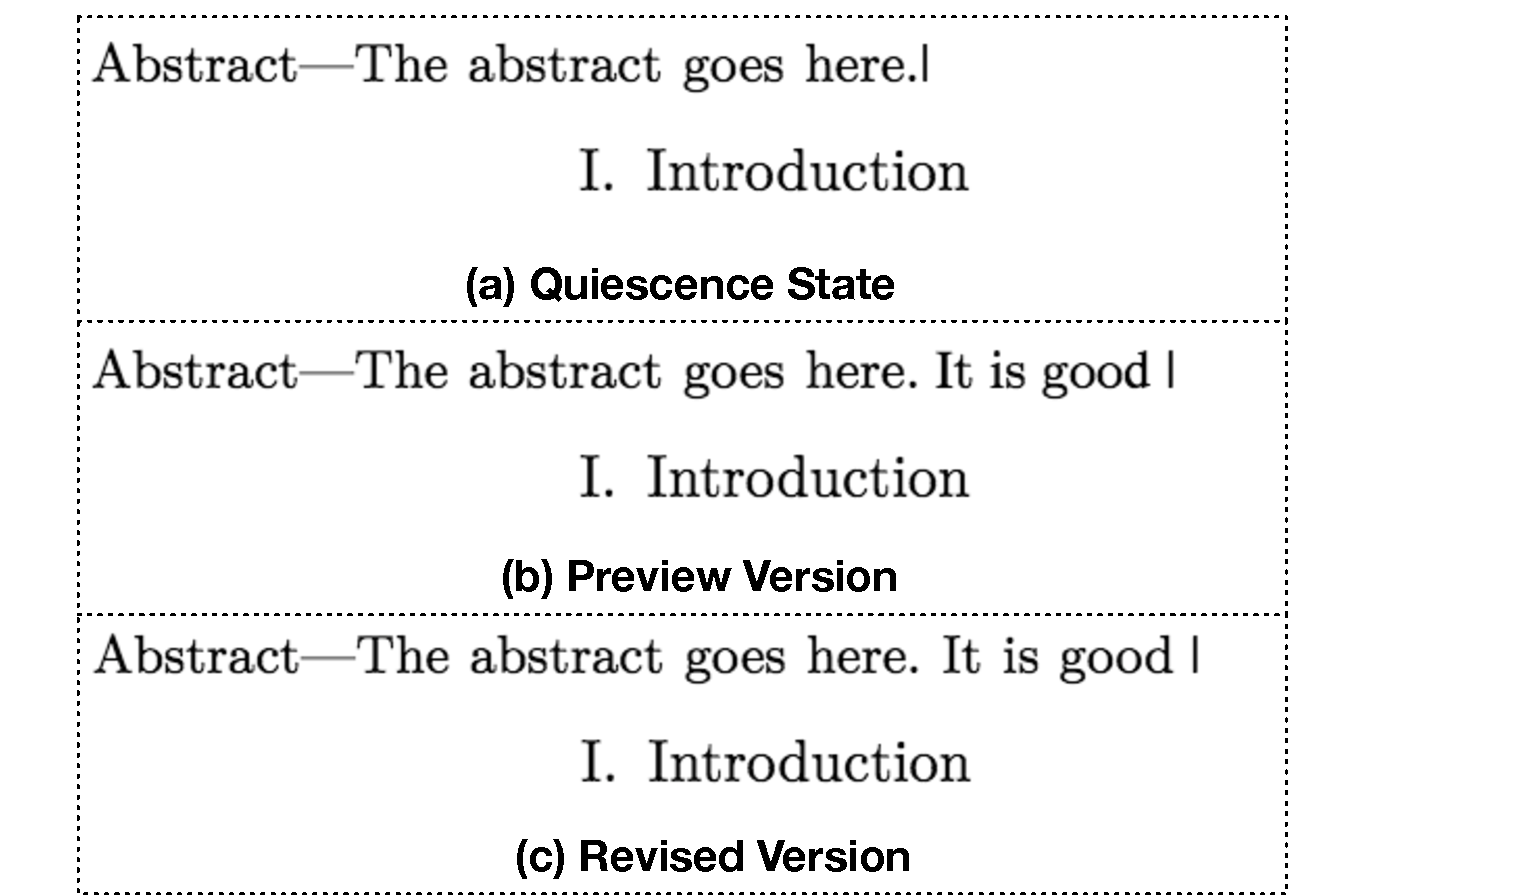
\includegraphics[width=0.40\textwidth]{figure/editing_example}
\caption{Three Editing States in the WYSIWYG View.}
\label{fig:editingexample}
\end{center}
\end{figure}

To provide an authentic experience of WYSIWYG editing, SwiftLaTeX puts considerable effort into generating a preview version that possesses minimal difference from the corresponding revised version as depicted in Fig~\ref{fig:editingexample} (b) and Fig~\ref{fig:editingexample} (c).
This is mainly achieved by mimicking the typesetting behavior used in the \LaTeX\ engine. 
For instance, when a character is being appended, it will automatically inherit the font settings from the previous characters to make itself visually agreeable.
Though the typesetting imitation approach is feasible for minor editing, it possesses certain limits when dealing with lengthy edits.
As a consequence, without any further precautions, the difference between the previewing version and the revised version would gradually accumulate along with the user's input.

To address this issue, one natural idea is to  compile the source periodically, and base the preview version on the newly-obtained revised version, such that the accumulated difference is cut back and remains unnoticeable most of the time. However, implementing such a mechanism entails a challenge, which is mainly attributed to the nature of asynchronous communication, \ie the fact that the user can keep on editing while a new version is already in the process of being compiled. 
We depict the predicament in Fig~\ref{fig:timingchart} (a) using a timing chart.
The chart contains two separate timelines. 
The topmost timeline indicates the period which the user spends on editing.
Likewise, the other timeline shows the timespan that the background compilation process consumes.
It can be observed that at the moment $t_1$, a background compilation request is initiated.
Meanwhile, since SwiftLaTeX is asynchronous, the user continues his editing regardless of the status of the background compilation process.
At the moment $t_2$, the compilation is finished and the revised PDF is available for display.
However, it should be noted that this revised PDF is an output of the source code at the moment $t_1$. 
It does not reflect the user's inputs within the timespan between $t_1$ and $t_2$, which are referred to as the \textit{uncommitted edit}.
As a consequence, directly displaying the newly-obtained revised version would erase the user's uncommitted edit  from the screen, and that would  obviously be inappropriate because the user's editing process would be severely disrupted.

\begin{figure}[t]
\begin{center}
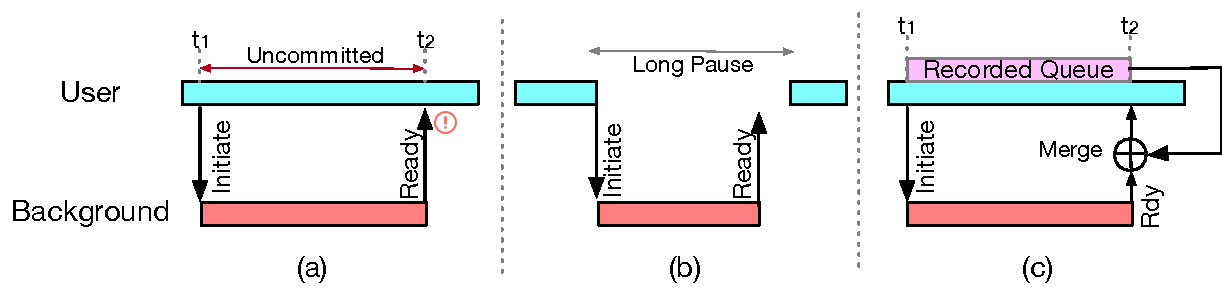
\includegraphics[width=0.5\textwidth]{figure/timechart}
\caption{Timing Charts in the WYSIWYG View.}
\label{fig:timingchart}
\end{center}
\end{figure}

One naive way to bypass this issue would be to take advantage of the user's pauses in editing as shown in Fig~\ref{fig:timingchart} (b). 
Specifically, it is not uncommon that a user occasionally takes a break from typing.
If such a break is detected, a background compilation would then be initiated.
If the compilation is finished before the user restarts his editing, the resulting PDF then can be safely displayed on the screen. This approach essentially uses the aforementioned concept of editing quiescence as a way to achieve consecutive safe updates of the PDF that do not interfere with the user input.
Nevertheless, this method is prone to starvation (i.e., long delay of the compilation process) if the user is typing swiftly and continuously for a long time.

Instead, SwiftLaTeX adopts a more sophisticated approach which does not rely on the user's pauses.
This is depicted in Fig~\ref{fig:timingchart} (c); the revised PDF, before being displayed in the viewer, is `merged' with the uncommitted edit so that the user's editing process will not be disrupted.
This can be achieved as follows.  
First, when the background request is initiated at $t_1$, our system starts recording all the editing operations in a queue data structure.
When the revised PDF is available at $t_2$, all the operations are dequeued  and replayed on the revised the PDF sequentially.
This generates a new preview PDF, which derives from the just-received revised PDF by adding the uncommitted edit.
Thus it is ready to be displayed in the viewer. The cursor is repositioned at the correct logical position in this new preview PDF and the user can continue editing without interruption.

\begin{figure}[t]
\begin{center}
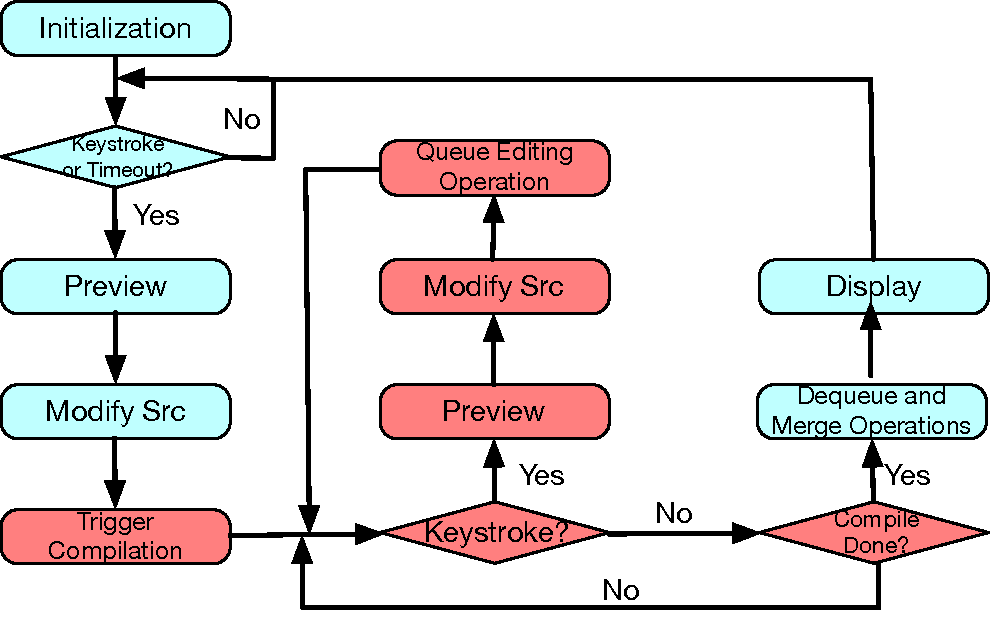
\includegraphics[width=0.40\textwidth]{figure/flowchart}
\caption{Workflow for the WYSIWYG view.}
\label{fig:flowchart}
\end{center}
\end{figure}


We summarize the aforementioned design with a flowchart shown in Fig~\ref{fig:flowchart}, where the blocks with ongoing compilation process are colored in red. A new compilation process will be triggered whenever either a keystroke or a timeout event (i.e., periodically trigger) is detected. This ensures that the users can obtain the latest revised version as soon as possible.



% Nonetheless, due to the complexity of the 
% It should be noted that though the foreseeing version is not guaranteed to be exactly the same as the revised version.





% % To demonstrate the predicament,  Figure~ depicts a timing chart of a random individual's editing process. 
% % The chart contains two separate timelines. 
% % The topmost timeline consists of the user's keystroke events. 
% % For demonstrate purposes, any two consecutive keystroke events that occur within a relatively short time interval (100 ms, the average typing interval of a novice typer []) are merged.
% % The resulting groups then are corresponding to a scenario when the user is inputing characters in a bursting manner. 
% % Between groups, pauses can be seen and indicate the timespan when the user is taking a rest from typing. 
% % The other timeline is for background complication process and is expressed in a waterfall view.
% % Noted that each sub-procedure in the background process is synchronous, in other words, only one sub-procedure can be executed at the same time.
% % It can be observed that at the $t_1$ moment, a background complication request is initiated. Meanwhile, the user decides to continue the writing process.
% % At the $t_2$ moment, the resulting PDF is retrieved from the network and delivered to the viewer for display.
% % It should be noted that the PDF is an output of the source code at the $t_1$ moment.
% % Therefore, its content does not reflect any user's inputs within the timespan between $t_1$ to $t_2$.

% % This issue does not severely impede the functionality of the conventional cloud-based systems, which decouple the editor from the viewer. 
% % Though the viewer is displaying the outdated PDF corresponding to the source code at the $t_1$ moment, the editor is in its correct state (i.e., contents and cursor positions at the $t_2$ moment).
% % Therefore, the user can either choose to continue editing without the viewer or pause awhile to await the latest PDF appearing on the viewer.

% % Nonetheless, the same issue cannot simply be  ignored in SwiftLaTeX. 
% % The main reason is that as a WYSIWYG editor, the viewing and editing are now intertwined. 
% % In other words, the PDF and the user's current edit (including typed characters and cursor positions) will be rendered on the screen simultaneously.
% % At the $t_2$ moment, the viewer is instructed to alternate the screen content with the dated PDF. It will also erase the user's edit between the timespan from $t_1$ to $t_2$.
% % The disappearance of the user's edit then prevents the user's from further editing.
% % it now simultaneously displays the compiled PDF and the user's input.
% % On one hand, it is in charge of displaying the compiled PDF. 
% % On the other hand, it also serves as an editor to accept the user's input, which will be immediately reflected by the viewer
% % Therefore, displaying an dated PDF leads to a side effect that certain recent input may disappear from the screen.

% % The viewer is not only displaying the PDF contents, but also indicating the input states like contents and cursor positions. Therefore, by displaying an outdated PDF, the input states are also sabotaged.




% % Displaying is straightforward to implement on conventional cloud-based systems, whose viewer is solely in charge of displaying and able to to alternate the display content at any time. However, the simplicity disappear in SwiftLaTeX's editable PDF viewer, where the change of display content also affects the input state of the user.

% % Specifically, the editor is able to accept any texts from the user regardless of the state of the viewer. Contrariwise, the viewer can alternate the display content freely without affecting the state of the editor.
% %  When the user enters texts, the state of the viewer change accordingly. 


% % However, in SwiftLaTeX, the editable PDF viewer possesses a more complex internal state.
% % Editing and viewing are intermingle.

%  % at the moment $t_2$


% % Meanwhile, the user continues his writing process. 



% % until the moment $t_2$ arrives. At this moment,  

% % Consider the moment $t_1$ when a background complication request is initiated. Afterwards, the user may decide to continue his writing process. At the $t_2$ moment, the resulting PDF is retrieved from the network and ready for display. 
% % However, the retrieved PDF is an output of the source code at $t_1$ moment. Thus, it is inappropriate to directly display the retrieved PDF, because it does not reflect any keystroke information with the timespan between $t_1$ and $t_2$. 



% To address this issue, one naive solution is to postpone the complication request until a user pause is detected. However, this approach is prone to starvation (i.e., long delay of the complication process) when the user is swiftly typing a long chunk of texts. As a consequence, the user's input is applied on a long-outdated PDF version. 
% % The chart contains two separate timelines. The topmost one consists of the user's keystroke events. For demonstrate purposes, any two consecutive keystroke events that occur within a relatively short time interval (100 ms, the average typing interval of a novice typer []) are merged and a group of keystrokes suggests that the user is inputing characters in a bursting manner. 
% The other timeline is for background complication procedures, 



% a waterfall chart . by separating the user's input timeline

% For instance, the user may decide to continue writing even a previous compilation is still progressing.
% Such a feature inevitably leads to a predicament depicted in Figure~. 


% To clearly demonstrate the predicaments, Figure~ depicts the timing view of a random individual's editing process. It should be noted that 


% In other words, the user is able to continue writing even a previous compilation is still progressing.
% In other words, 




% Therefore, Figure depicts two separate timelines; one for the user's keystroke events, the other one for the network operations. For demonstration purposes, any two consecutive keystrokes that occur within a relatively short time interval (xx ms, average typing interval of a novice typer []) are merged and a group of keystrokes suggests that the user is inputing a burst of characters. 

% The challenging issue lies on the the fetch PDF does not contain the dirty content.
% % the keystroke events are clustered into groups, where any two consecutive keystrokes . 

% For demonstration purposes, the keystroke events are clustered into groups, where any two consecutive keystrokes occur within a relatively short time interval (xx ms, average typing interval of a novice typer []). Thus, the existence of a group suggests that the user is inputing a burst of characters. 
% Between groups, pauses can be seen and indicate the timespan the user takes to think about what to write next.

% Given such a timeline, two questions arise naturally, namely 1) when to trigger a background compilation process and 2) how to display the product of the recent compilation. 

% Regarding the first question, an intuitive solution is to trigger complication whenever a pause is detected. 
% However, this approach is prone to starvation (i.e., long delay of the complication process) when the user is swiftly typing a long chunk of texts. 
% Another straightforward solution is to trigger complication if a keystroke is detected and there is no going complication task.
% Though this approach prevents the starvation, it is likely to induce a latency problem when the cloud server is experiencing a heavy load. This scenario is depicted in Fig where a user is typing a word `abcde'. At the very beginning, the stroke `a' starts the first complication task. Assume typing this word takes $0.5$ second while the complication task consumes $3$ seconds due to heavy load. 
% Then the stroke `e' will trigger the second complication, which consumes another $3$ seconds. Therefore, the overall latency is $6$ seconds.

% Nevertheless, it is possible to optimize to latency by only sending one complication request when the user finishes typing the word. In that case, the overall latency is solely $3.5$ seconds, which is almost 50\% reduction.







% The two questions are non-trivial due to the asynchronous nature. Specifically, the user is entitled to decide when to edit texts regardless of the status of other background operations (e.g., compiling source codes and fetching resulting PDFs).
%The two questions are relatively trivial in the conventional cloud-based systems,


\section{Achieving Fine-grained Source Code Positioning}  \label{sect:textpos}
A WYSIWYG editor that synchronously changes the source code  requires a very finegrained ability to reconstruct the source code position of each element in the PDF.

\subsection{Inferring Source Code Positions}
As a WYSIWYG editor, SwiftLaTeX intercepts the modification on PDF elements (e.g., words or equations) and directly applies the corresponding alternation on the source code. To achieve this, SwiftLaTeX is required to infer the source code position of the modified PDF elements. 
Such an ability is commonly referred to as \LaTeX\ input-output synchronization, and this has been explored by a \LaTeX\ plugin named Sync\TeX. 

Sync\TeX\ is  designed for conventional typesetting editors, which usually incorporate two views; 
one for entering \LaTeX\ source code, the other for viewing the resulting PDF. 
Generally, the source code and PDF are too long to fit a window and thus only certain parts of the contents are visible to a user. 
To facilitate the user's editing process, the two windows are required to be synchronized such that they are displaying roughly the same part of the document. 
Solely taking this use case into account, the author of Sync\TeX\ deems it sufficient to provide line-level accuracy, which allows mapping from a PDF element to a whole line in input files \cite{laurens2008direct}. 
This coarse-grained accuracy is unable to meet the requirement of SwiftLaTeX. To address this issue and to boost the synchronization accuracy from line-level to at least  word-level, we have developed and tested two different approaches: first, we have developed an advanced text-matching approach. Secondly, we have enhanced the \TeX engine to achieve on demand even character-wise synchronization.


\subsubsection{Text-Matching Approach}

\begin{figure}[t]
\begin{center}
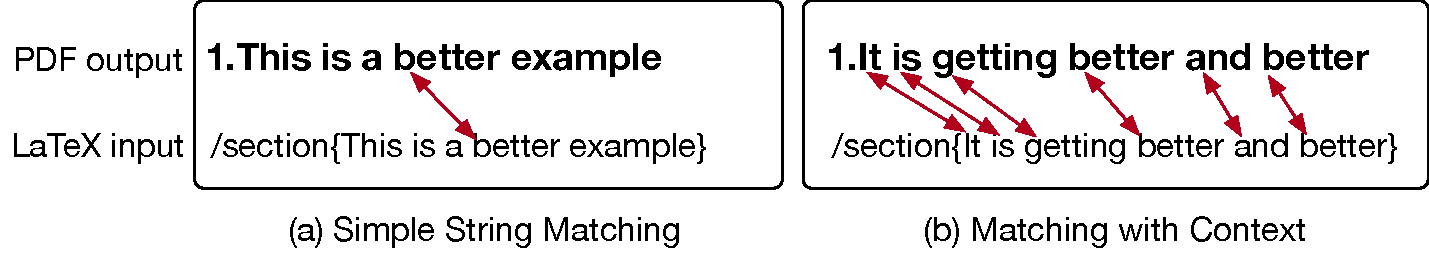
\includegraphics[width=0.42\textwidth]{figure/charmapping}
\caption{Two typical examples for source code position inference.}
\label{fig:char}
\end{center}

\end{figure}
For a better understanding of the text matching approach, Figure~\ref{fig:char} depicts two typical cases, each of which contains one line of \LaTeX\ source code and its corresponding PDF output obtained by Sync\TeX. 

Consider the first case in Fig~\ref{fig:char} (a) where we wish to infer the source code position of the word `better' in PDF. 
A straightforward solution is to run string matching algorithms on the line of source code, which reveals the correct position. 
However, this approach may cause ambiguity if the word `better' occurs more than once in a sentence as shown in Fig~\ref{fig:char} (b).
This exception naturally motivates us to take the surrounding words (i.e., context) of the target into consideration, more specifically, matching a sequence of words instead of an individual target.
%Specifically, instead of focusing on an individual target word, it is more reasonable to match a whole sequence of words simultaneously as it usually alleviates the ambiguity. 
This serves as the intuition of our approach to solve the source code position inference problem formulated as follows.

Given two character arrays $L$ and $P$, which represent a line of \LaTeX\ source codes and its corresponding PDF output string respectively. 
Besides, $L_j$ denotes the $j$-th character in the array $L$ and $ 1 \le j \le $ $len(L)$. 
Likewise, $P_k$ represents the $k$-th character in the array $P$ and $ 1 \le k \le $ $len(P)$. 
A matching $f$ between $L$ and $P$ is defined as a function that satisfies 
\begin{equation}
P_k = L_{f(k)}  \quad \quad \forall k \text{ in } [1, len(P)].
\end{equation}
Here we safely assume every character in $P$ has its matching on $L$. 
If there exists no matching for a specific character (e.g., the numbering characters in section header), we simply mark it as uneditable and remove it before proceeding. 

Meanwhile, we say a matching is valid if it is monotonic, which can be illustrated as follows.
\begin{equation}
f(i) < f(j)  \quad \text{iff } 1 \le i < j \le len(P).
\end{equation}
This property guarantees that the order of the characters in $P$ is also preserved in $L$.


Multiple matching may occur and we denote the fittest matching $f_b$ as the one which satisfies the following requirement:
\begin{equation}
f_b = \argmin \sum_{2}^{len(L)}(f(k) - f(k-1)),
\end{equation}
where $f$ represents a valid matching.
This requirement contains a simple intuition; for two consecutive characters in $P$, the distance between their matching characters in $L$ is also minimized under the fittest matching $f_b$. 


It can now be easily seen that the answer of the source code position inference problem happens to be the fittest matching $f_b$.

It is not difficult to obtain this mapping even in a brute-force manner considering the search space has already been greatly limited in a line of source codes.
Moreover, the search space can be further reduced by certain optimizations. For instance, the string matching algorithm can be first utilized on words that only occur once to immediately confirm their matching. 

Nevertheless, such an approach is still prone to matching failure. 
The main culprit derives from the precision of the Sync\TeX, which is $\pm 1$ line \cite{laurens2008direct} in most cases. 
The precision significantly degrades when the element is generated by a \LaTeX\ macro (e.g.,  math equations or section headers). 
Clearly, the incorrect line number negatively impacts the reliability of our approach.

The unstable technique now forces us to develop a more sophisticated approach, which increases the synchronization accuracy from the internal perspective of \LaTeX\ engines.

\subsubsection{Enhancing \TeX\ Engine}

\begin{figure}[t]
\begin{center}
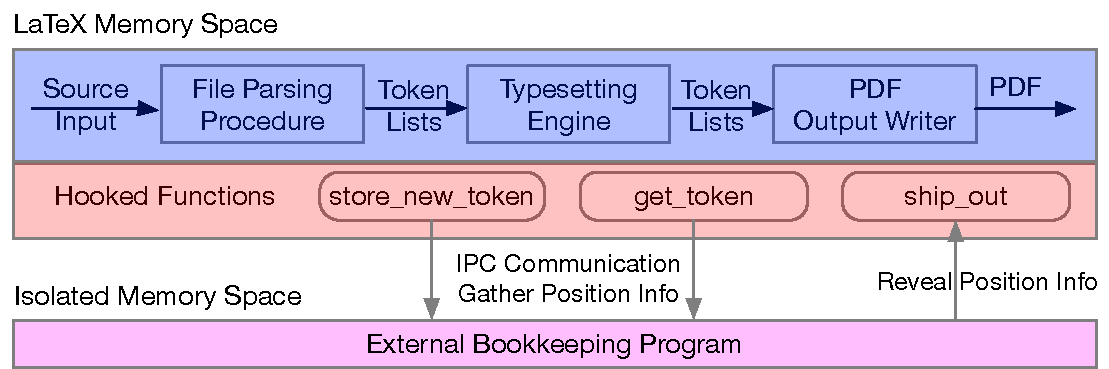
\includegraphics[width=0.42\textwidth]{figure/patchengine}
\caption{Internal Mechanism of the Engine Patch.}
\label{fig:enginepatch}
\end{center}

\end{figure}

%Original \LaTeX\ engines, when processing input files, possess no bookkeeping mechanism to handle the source code positions
Existing open-source \LaTeX\ engines possess no mechanism for tracking down the source code positions for each PDF element. 
In this work, we make the first attempt to enhance the engines with a bookkeeping mechanism that provides character-level synchronization accuracy.

The main challenge of implementing such a functionality lies in how to minimize the potential interference which our modification creates to the engines. 
Specifically, the original implementation of the \TeX\ engine is generally considered very complicated code that is difficult to modify in a safe way.  
Directly patching this source code  to alter the internal data structures or execution logic is considered not advisable from a standpoint of software reliability engineering, because an under-optimized patch is likely to result in unheeded bugs.
Therefore, to avoid undermining the reliability of \LaTeX\ engines, we adopt a neutral observer design in our patch as depicted in Fig~\ref{fig:enginepatch}.

It can be seen that the patch is partitioned into two essential parts. The first one is an external bookkeeping program. 
This runs in its own memory space and passively receives the position-related information from the \LaTeX\ engines in file parsing and typesetting phrases.
The information is obtained by the second part of our patch, which is a dynamic hooking library. 
In short, hooking is the process of intercepting a program's execution at a specific point, typically entries of functions, in order to augment the program's behavior. 
The binaries of the augmented functions are placed on a dynamic hooking library, which can be injected into \LaTeX\ engines' memory space via special instructions to program linkers on the run-time. 
The merit of the hooking technique is its unintrusiveness; neither modification nor re-compilation of the original source codes is ever required. 
Moreover, the augment functions in our patch does not alter the memory content of the \LaTeX\ process. The neutral observer design ensures the reliability is untarnished.

For better understanding of how the bookkeeping patch keeps track of the source code positions, it is reasonable to first introduce the procedure that \LaTeX\ engines utilize to parse input files. Briefly speaking, \LaTeX\ digests the input files character by character. 
These characters are generally stored and organized in a data structure named \textit{token lists}, which are essentially linked lists. 
A token list can represent a character array to be printed or a parameter for a macro call (e.g., `Paper' in $\backslash$title\{Paper\}). 
Depending on the implementation of the macros, a parameter token lists can be moved around in the memory by being duplicated and removed several times before they are finally formatted and printed on PDF.

Therefore, to establish a mapping between the source code positions in input files and their output elements in PDFs, two essential steps are involved. 
The first step is to build and attach a position record for every constructed token list when processing input files. 
The immediate step is to ensure the position record can be propagated to its newly duplicated token lists. 

To implement the two steps, at first glance it would appear unavoidable to modify the data structure of the token list such that it can store the source code position. 
However, our patch is able to avoid this by  adopting a significantly different approach. 
Specifically, the patch hooks two functions including 1) \textit{store\_new\_token()} and 2) \textit{get\_token()}. 
The former function  is used to dynamically allocate the memory space for a new token being appended to a token list. 
The latter function, on the other hand, may be used to retrieve a token from memory for duplication. 
These functions are now augmented such that the memory addresses and contents of the newly allocated token or the recently retrieved token will be delivered to the external bookkeeping program via inter-process communication channels. 
Meanwhile, if a token is constructed when parsing input files, the corresponding source code position is also delivered. 

By monitoring the memory data received, the external program now can keep track of every token list and its associated position record. 
The maintained information will then be utilized in the hooked \textit{ship\_out} function at the PDF output stage.
Specifically, if a token list is being printed on PDF, the external program will simultaneously reveal the associated position information, which may be stored in the following approaches.

\subsection{Storing Position Information}
With the enhanced \LaTeX\ engine, every PDF element is now associated with its source code position. The remaining question lies on how to store the position information such that it can be easily retrieved by a viewer.

A first solution is to follow Sync\TeX , which takes advantage of an auxiliary file. 
Specifically, the file serves as a dictionary which maps the coordination of PDF elements to their line numbers; whenever a user clicks a specific PDF element on the viewer, the mouse coordinates can be checked against the auxiliary file to obtain the corresponding line number. 
Clearly, the principle can be easily adapted in our work. 
However, one drawback of this solution stems from the specifically-designed auxiliary file, which can only be parsed by a unique external program \cite{libsynctex2011}. It negatively impacts the portability of PDF files.

Alternatively, we propose a novel approach which directly embeds the position meta information to the PDF files. 
The merit of this approach is that it allows viewers to retrieve the positions without the auxiliary file and external program. 
Nevertheless, the implementation entails an inevitable challenge that the PDF specifications do not take synchronization into consideration and there exists no generally-acknowledged approach for storing the position information on a PDF file. 

To tackle this issue, we explore an idea that piggybacks the position information on undocumented PDF metadata. 
Specifically, PDF metadata is utilized to describe properties such as the font, shape and position of a PDF element. 
Among them, a property named \textit{flatness} is barely documented by the PDF specification \cite{libpdf2008}. 
We investigate how this property is handled via cross-checking various open-source PDF viewers such as Poppler\cite{libpoppler2008} and Evince \cite{libevince}. 
The results indicate that all of the viewers simply ignore this property when rendering a PDF on screen. 
In other words, the flatness property can be stored as any value without impeding the functionalities of the viewers. 
Therefore, we piggyback the position information on the flatness property.
In this manner, whenever a user clicks a PDF element, its flatness property can be retrieved and utilized  by a viewer to infer the source code position. 
Note that since almost every PDF viewer possesses graphical or programming interfaces for directly accessing the metadata, neither external program nor patch for viewers is required. 

Despite its promising feature, we have to admit that the piggyback approach indeed contains a minor drawback; the size of the resulting PDF is slightly bloated due to the extra flatness property. 
Nonetheless, this side effect is negligible thanks to the PDF stream compression mechanism \cite{libpdf2008}, which greatly reduces the redundancy of the position information. 
%Moreover, the user can switch off the piggyback option at ease such that the size of the final PDF is not affected. 
Moreover, the piggyback option can be  switched off easily when the user decides to publish the final version of the PDF.
% To hold the line and column number simultaneously, we encode them to using mechanism.

% We admit that such an approach indeed contains two minor drawbacks. First, 


% it bloats the size of PDF file. 
% Second, it only supports limited number line and column. \todo{Do some discussion}


% Moreover, the hooking library can be uninstalled in real-time if it is causing instability to the original program. 


%In summary, the design of our patch does not alter any memory contents of the original \LaTeX\ programs such that their reliability is untarnished.
% A hooking library containing  can be dynamically injected to an application via instructing linkers from the operating systems.








\section{System Implementation}\label{sect:imp}
In this section, we present the implementation details of SwiftLaTeX and showcase its main user interfaces.

\subsection{Achieving High Scalability and Reliability}
As a cloud service designed for a large number of potential users, SwiftLaTeX aims to meet demanding requirements for scalability and reliability.

\begin{figure}[t]
\begin{center}
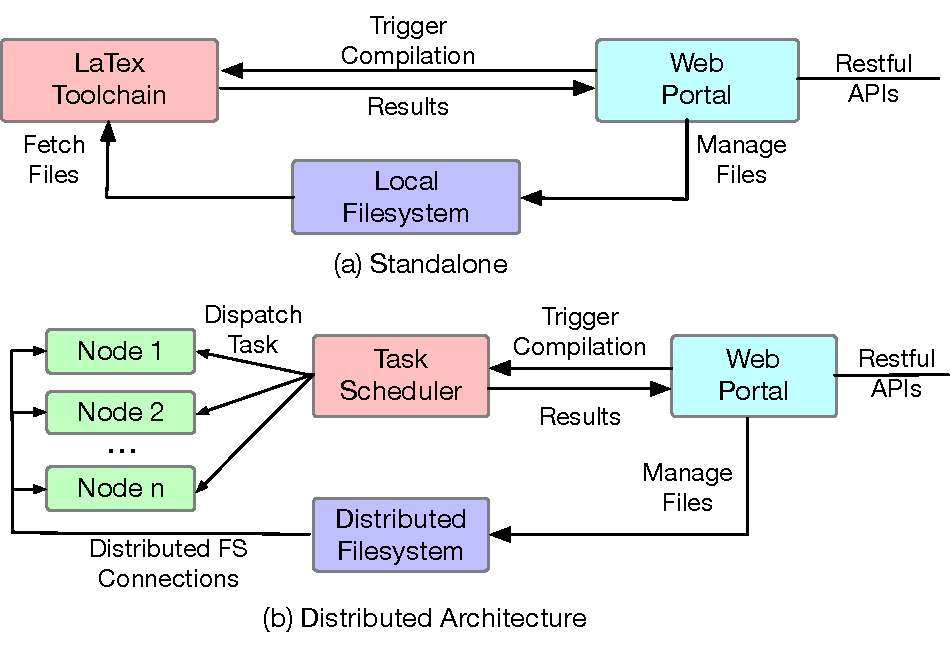
\includegraphics[width=0.40\textwidth]{figure/cloudarchitecture}
\caption{Backend Architectures.}
\label{fig:cloudarch}
\end{center}

\end{figure}


To understand the challenges, let's discuss a prototype running on a single server.
 As shown in Fig~\ref{fig:cloudarch} (a), the prototype contains two components, a web application and a \LaTeX\ toolchain. The web application offers a set of restful endpoints enabling users to upload their \LaTeX\ source code to the server. 
 These files can be processed by the \LaTeX\ engine to generate the resulting PDFs. 

Despite the simplicity, an obvious drawback of this single-server prototype lies in limited system capacity. More specifically, the performance bottleneck can be mainly attributed to the time-consuming compilation process, and the hence limited number of compilation tasks that can be run on a single server concurrently.
  Another major limitation of  this single-server prototype is its questionable reliability. If the prototype  stores all users' files solely in its local hard disk, then the failure of the hard disk can create a single point of failure, resulting in data loss or system unavailability. 


% Moreover, such a prototype possesses questionable reliability since it is prone to the single point of failure. 

To address these issues, SwiftLaTeX replaces this prototype with a sophisticated distributed architecture as shown in Fig~\ref{fig:cloudarch} (b).
One major enhancement is providing support for scale-out. 
Specifically, instead of executing all the compilation tasks on a single host, the distributed architecture now is able to dispatch different tasks to multiple hosts named \textit{compilation nodes}. Such a design not only ensures the scalability by incorporating additional nodes, but also enables optimization of the system latency by applying scheduling algorithms on different types of tasks. 
Currently, SwiftLaTeX schedules the compilation tasks by adopting a Multilevel Queue approach inspired by the process scheduling in modern operating systems \cite{silberschatz2014operating} .
Briefly speaking, compilation tasks are first assigned with a priority (e.g., high, medium and low) based on the length of the source code.
Afterwards, the tasks with an identical priority will be dispatched to the same compilation nodes in a first-come-first-served manner. 
Compared with a randomized scheduling mechanism, this scheduling algorithm is highly likely to reduce the average latency, since it alleviates the convoy effect that a time-consuming task holds other simpler tasks for a long time \cite{lee2011improving}.
This also mitigates the problem that none of the existing \LaTeX\ engines takes advantage of multi-core processing.


Also the architecture significantly increases the system reliability by utilizing distributed file systems. 
Specifically, files are now replicated and scattered across multiple hosts, such that despite the failure of a small number of hosts, the data would remain intact and available.
Another advantage of distributed file systems is the intrinsic support for file version control. It greatly facilitates the implementation of Version Control Systems (VCS) in SwiftLaTeX, which allow users to straightforwardly manage the change of their \LaTeX\ source codes.
% Meanwhile, SwiftLaTeX also benefits from the file version control functionality in the distributed file system. In details, the file system now keeps track of every modification of a file.

SwiftLaTeX implements the above mechanisms with the help of open-source components including Redis Queue \cite{carlson2013redis}, GridFS \cite{banker2011mongodb} and Docker \cite{merkel2014docker}. 
Specifically, Redis Queue is used to implement the task queues for each compilation node. Meanwhile, their hard drives are all connected to form the distributed file storage using GridFS. To facilitate fast deployment, the entire SwiftLaTeX is packaged into a Docker image format, which is a de facto standard used by various cloud computing platforms.

% is a distributed data structure store, commonly used as a message broker. To facilitate simple deployment, SwiftLaTeX adopts the Docker technique, which encapsulates all the used software components in a universal image. Such an image can be easily hosted in various kinds of cloud-platforms. 


\subsection{Embracing Responsive Frontend Design}
To ensure the compatibility (i.e., being responsive) to mainstream browsers running on various kinds of devices such as desktops and tablets, SwiftLaTeX is solely built atop the standard front-end technologies including HTML5, CSS3 and Javascript. 
Nonetheless, these technologies are supported to a different extent by each browser and different browser version. 
The differences pose a main challenge to the frontend design, notably, rendering PDF correctly  in the WYSIWYG view across various browsers.


\begin{figure*}[t]

\begin{center}
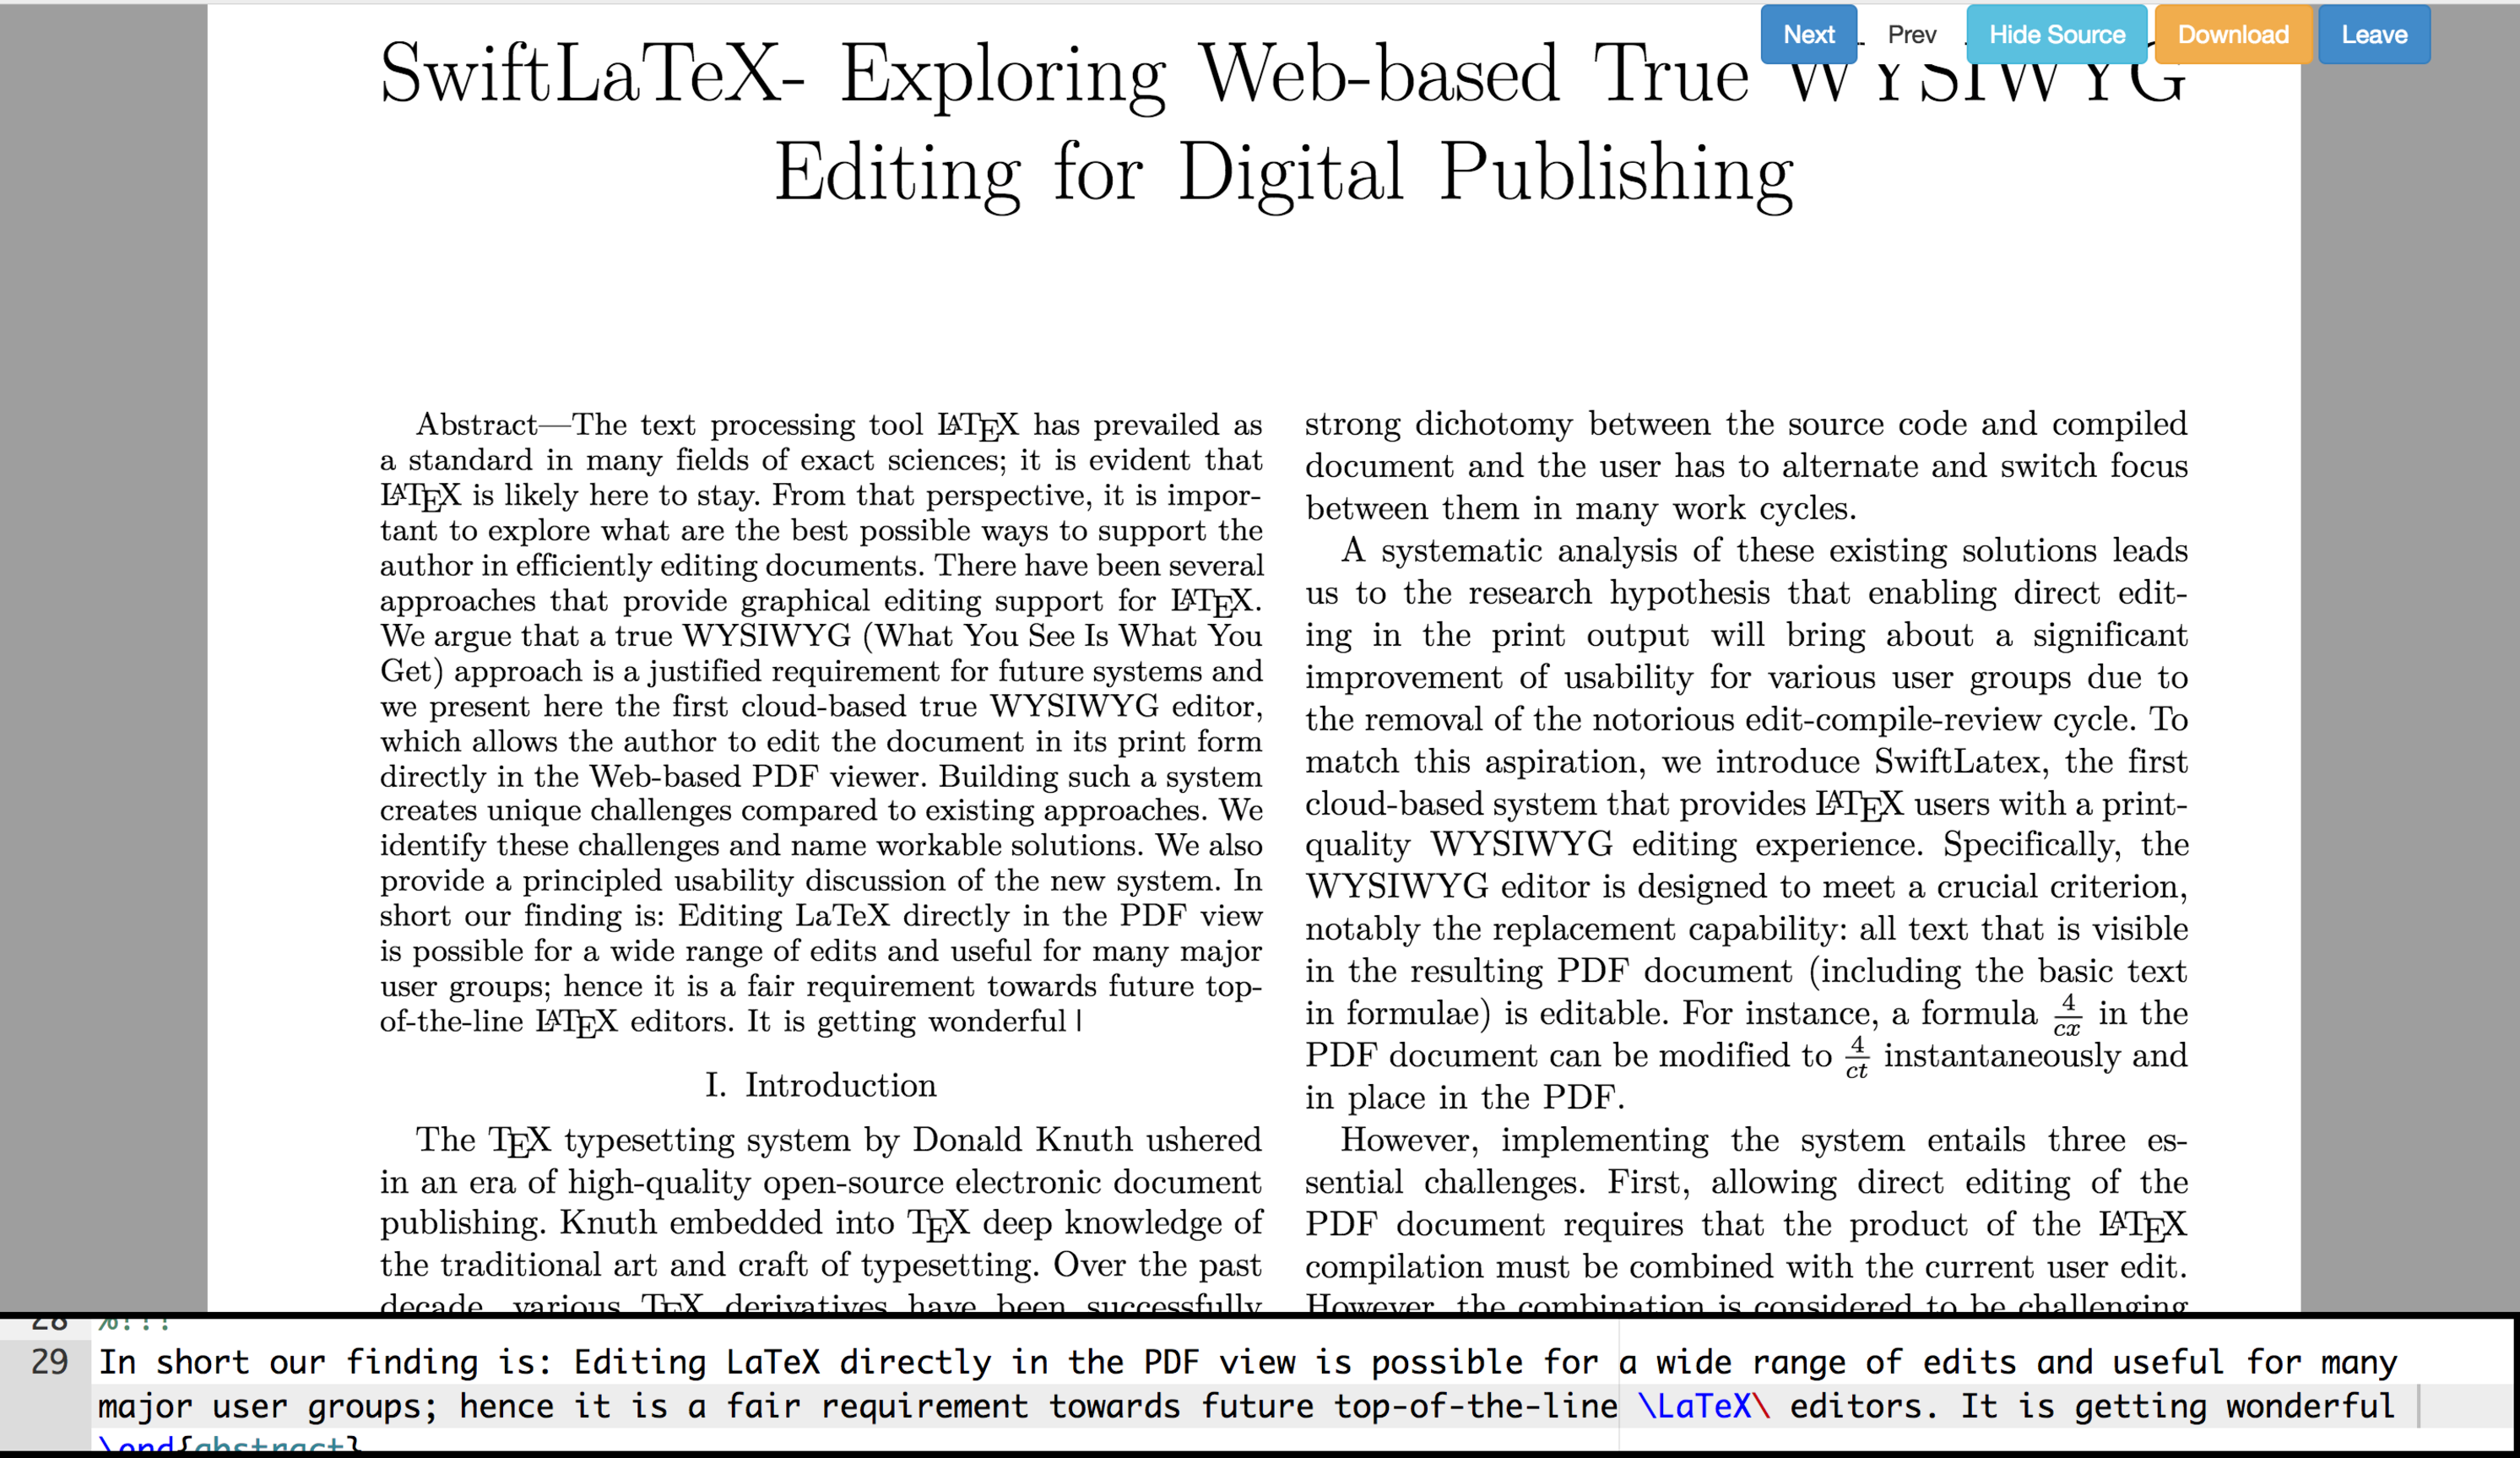
\includegraphics[width=0.90\textwidth]{figure/screenshot}
\caption{WYSIWYG Editor of SwiftLaTeX}
\label{fig:screenshot}
\end{center}
\vspace{-0.1in}
\end{figure*} 

Specifically, each browser has its own setting to control how PDFs open from a webpage. 
Browsers such as Internet Explorer or Opera display the PDF by invoking an external PDF reader (e.g., Adobe Reader), which is not always available.
Though a small number of browsers like Chrome possess built-in PDF readers, their functionalities are commonly limited (e.g., previewing PDF in an independent browser window). 
It is generally difficult for SwiftLaTeX to integrate and extend them due to the lack of application programming interfaces (APIs).
To tackle this issue, SwiftLaTeX explores two different approaches including a Javascript-based PDF viewer and a plugin for the \LaTeX\ engine to generate HTMLs instead of PDFs.

The first method takes advantage of \textit{PDF.js} \cite{pdfjsintro}, a Javascript library for parsing and rendering PDF atop the canvas of a browser window. Despite the straightforward setup, the library is likely to experience performance issues (e.g., slow rendering) when processing PDFs with substantial pages. It is mainly because Javascript, as an interpreting language, is not performance-oriented especially on the resource-constrained mobile devices. Moreover, PDF.js is known to have compatibility issues with certain browsers such as Internet Explorer and WebKit used in earlier versions of Android \cite{pdfjs}.

The second approach is inspired by a library named \textit{Pdf2htmlEX} \cite{wang2013online} that converts PDFs to HTML5 pages.  
The conversion is carried out in an manner that all the texts, figures, mathematical formulas and page layouts are preserved with precise fonts and locations. It ensures that the visual difference between PDF and HTML is barely noticeable.
SwiftLaTeX adopts the core idea and serves HTMLs rather than PDFs to users. The essential merit lies in its high compatibility and tiny resource consumption.
 In particular, the HTML pages can be directly displayed by most browsers and the process only consumes a tiny amount of CPU and memory resource. It makes SwiftLaTeX more friendly to resource-constrained devices.

% TODO: This would probably need more explanation and would currently go too far.
%Nevertheless, SwiftLaTeX does not rely on Pdf2htmlEX to convert PDFs to HTMLs. The main reason is that the conversion is inefficient due to the unnecessary detour (from \LaTeX\ sources to PDFs, then from PDFs to HTMLs). Instead, SwiftLaTeX implements a plugin to enable the \LaTeX\ engine  to skip the intermediate PDF step and to generate HTMLs from \LaTeX\ sources directly.

SwiftLaTeX consolidates the technologies mentioned above and implements a user interface as shown in Fig~\ref{fig:screenshot}.
We reuse a set of responsive open-source components, for example, Bootstrap \cite{spurlock2013bootstrap} to provide a responsive layout, jQuery \cite{bibeault2008jquery} to manage restful connections with the backend, and Ace.js \cite{acejs} to provide syntax highlighting in the source view.
% Nevertheless, the library requires browsers to have a comprehensive support of HTML5, which may not be available in certain resource-constrained devices.
% In contrast, the second approach preprocesses the PDF and converts it to HTML files. The main advantage is that it is friendly to resource-contrained devices. Moreover, it reduces the implementation difficulty of front-end design.
% it is easier to alter the contents residing the DOM tree compared with in the canvas.




% Although the majority of browsers provide PDF viewing functionality, it is quite limited and not flexible.
% One essential component of the user interface is the PDF viewer. 
% SwiftLaTeX utilizes two different approaches to display PDF. The first one is through a javascript library named \textit{PDF.js}.
% PDF.js is a PDF viewer that is built with HTML5. 
% However, such a approach handle drawing directly.
% The second approach relies on our experimental \LaTeX\ engine, which directly outputs HTML files.



% \textbf{Math Formula Editor} 

% \textbf{Table Editor}
% \LaTeX\ tables are a powerful and commonly-used feature.
%  However, its sophistication generally poses a significant barrier to  novice \LaTeX\ users.
%   To alleviate the difficulty of mastering \LaTeX\ tables, SwiftLaTeX offers users with a graphical \LaTeX\ table generator as shown in Fig.
%    The tool allow users to specify the row/column number of tables and to alter the properties (e.g., contents, or border width) of each table cell in a spreadsheet-like interface. 
%   Once the editing is finished, the generated table can be inserted to a user-specified location in the PDF viewer.


% \textbf{Optimization for E-reader Devices}
% \todo{probably not?}
% E-reader devices are gaining in increasing popularity recently.
% To enable document editing on the e-reader devices, SwiftLaTeX adopts several optimizations.




\section{Prototype Evaluation}\label{sect:eve}
To evaluate the usability of SwiftLaTeX, we invited 6 participants from the academic domain to test our system. 
The evaluation has been organized as a Discount Usability Test \cite{nielsen1989usability}, which involves a small number of participants with a focus on qualitative studies on prototype design. Previous studies \cite{nielsen2015you}\cite{nielsen2009discount} have suggested that a discount usability test, even with only 5 participants, provides robust evaluation results and may discover up to 85\% of the 
usability problems. In this section, we demonstrate the settings and outcomes of our evaluation. 
The preliminary test offered us many invaluable insights and feedbacks.
In the near future, we plan to perform a comprehensive usability study, which covers more participants from different domains.

\subsection{Evaluation Settings}
We invited 6 participants, who are Ph.D. candidates and Postdoctoral researchers from various disciplines such as Computer Science and Geo-Informatics, to attend our evaluation session.

Before undertaking the test, each subject was requested to complete a short questionnaire about their background knowledge and skills in using \LaTeX. Specifically, we required each participant to answer the following two categories of questions on a five-point scale (strongly disagree, disagree, neutral, agree, strongly agree):
\begin{itemize}
\item Knowledge about \LaTeX\ script language.
\item Experience in using \LaTeX\ editors (either online or standalone).
\end{itemize}

Afterwards, the participants were instructed to perform the following tasks in an unsupervised manner; the subjects were required to finish the tasks on their own without any prior knowledge of SwiftLaTeX.
\begin{enumerate}
	\item We instructed each participant to compose a paragraph with approximately 200 words to describe their current research interests. 
	\item We offered each participant with one English paragraph on a topic of general interest. In each line of the paragraph, there exists an obvious typo and the participants were required to correct it.
	\item We provided each subject with a set of simple mathematical equations with incorrect calculation (e.g., $1 - \frac{1}{4} = \frac{2}{4}$). The participants were required to correct the final results of the equations.
\end{enumerate}

After completing the aforementioned tasks, we asked the participants to fill in a System Usability Scale (SUS) questionnaire, which is a widely-used reliable tool for perceived usability evaluation even with a small sample size \cite{brooke1996sus}.
We also requested participants to report their experience of using SwiftLaTeX.

\subsection{Evaluation Outcomes \LaTeX{}}


\textbf{SUS Score.}
The mean SUS score of SwiftLaTeX is 78 (in a range spanning from 0 to 100). It exceeds the threshold score of 68 which  indicates a decent level of usability \cite{brooke1996sus}. 
In addition, as suggested by the research \cite{lewis2009factor}, we also compute the mean values for the usability sub-scale and learnability sub-scale, which are 74 and 91 respectively. 

Meanwhile, by considering participants' answers given in the background questionnaire (i.e., Knowledge of \LaTeX\ language and Experience in \LaTeX\ editors), we obtain two more background sub-scores.
They are compared with the SUS score and sub-scale scores to obtain the Pearson correlation coefficients. 
We notice a weak negative correlation between the two background sub-scores and the learnability score, which may imply that a novice \LaTeX\ user may find it easier to master our system.
However, due to the small sample size, each correlation measure appears to be not statistically significant. To reach a more solid conclusion, a more comprehensive dataset is required.
% All the 6 participants actively responded to our invitation and we received 6 responses about the current prototype of SwiftLaTeX.

\begin{table}[]

\centering

\caption{Axial coding of the participants' comments on SwiftLaTeX}
\label{tab:comments}

\begin{tabular}{|l|l|l|}
\hline
Categories                                                      & Positive & Negative \\ \hline
\begin{tabular}[c]{@{}l@{}}WYSIWYG\\ Editing\end{tabular}       & 6        & 2        \\ \hline
\begin{tabular}[c]{@{}l@{}}In place\\ Math Editing\end{tabular} & 6        & 0        \\ \hline
Efficiency                                                      & 6        & 0        \\ \hline
Web-based                                                       & 3        & 0        \\ \hline
Hotkey                                                          & 0        & 4        \\ \hline
Synchronization                                                 & 1        & 0        \\ \hline
Learning Curve                                                 & 1        & 0        \\ \hline
\end{tabular}

\end{table}

\textbf{Feedback.} All the participants' comments are summarized in Table~\ref{tab:comments} using Axial coding \cite{strauss1990basics}. 
On one hand, the positive feedback is mainly attributed to 1) innovative WYSIWYG editing for basic text and mathematical formulas, 2) the web-based interfaces, and 3) high efficiency for various kinds of editing tasks such as proofreading. 
A participant also provides valuable insight into the benefit of fine-grained synchronization.
Specifically, existing \LaTeX\ editors behave poorly in proofreading tasks mainly because of the coarse-grained synchronization functionality. 
A word in PDF is commonly mapped to a lengthy line in the source code.
 To modify the word, users are required to skim through the line to get the exact position of the word, which is fairly time-consuming. SwiftLaTeX successfully overcomes this issue by achieving character-level synchronization accuracy.
Another participant who has little experience in \LaTeX\ applauded the smooth learning curve of SwiftLaTeX, which possesses high familiarity with the existing word processors but produces much more high-quality typesetting output.
In addition, SwiftLaTeX allows users to focus on document composition without concerning about the complex script language and the time-consuming compilation and debugging process.

On the other hand, Table~\ref{tab:comments} also reveals some widely perceived issues. Specifically, one important issue highlighted was the rudimentary functionality to conduct structural changes (e.g., adding a new section or list structure). 
Currently, these structural changes could be applied via clicking the corresponding options in the context menu (i.e., pop-up menu).
However, one subject suggested that it would be more helpful if SwiftLaTeX could mimic the autoformat features (e.g., automatic bullets or numbering) from the word processor. 
Alternatively, SwiftLaTeX could support Markdown language such that a simple snippet could be used to generate structural changes.
Meanwhile, the majorities of subjects also complained about the invalidity of commonly used hotkeys (e.g., control + c). Another report also reveals that the delete key is not working properly.
% The main culprit of these flaws lies in a non-fatal compatibility issue of different browsers which possess different key handling mechanisms. Therefore, some functional keys may trigger inconsistent Javascript events in different browsers.

% is mainly attributed into coarse-grained synchronization accuracy. When a user plans to change a single character in PDF, the synchronization functionality only highlights one lengthy line on the source code. Thus, the user has to skim through the line to get the exact corresponding position.
	
\section{Further Discussions}
SwiftLaTeX shows the potential for web-based WYSIWYG editing for \LaTeX. Still, it bears several limitations that need further improvement.

\subsection{Enabling Hotkeys and Clipboard}
The implementation of clipboard features such as cut/paste was only postponed due to project management reasons and is one of the next straightforward development steps. With the architecture of SwiftLaTeX it is easy to achieve cut/paste even of structural elements such as section headers. This offers a further option for users to perform structural edits. 

\subsection{Facilitating Structural Edits}
Finding a natural interface for structural edits is a challenge to WYSIWYG tools. 
Many tools support structural edits primarily as inserts with a large number of menus or analogs of often hard-coded menus. 
%It is our aim to provide a solution that is more principled. For inserts of structural elements such as headers, tables, bullet lists and more, we want to allude to the copy-paste function. 
Our design is a menu showing small pre-defined \LaTeX snippets that are examples of the needed elements. For example for a header the snippet could be "{\small \verb$\subsection{Sectiontitle}$}"  and in the menu this is shown in its compiled version. If the user selects the snippet, essentially a paste (insert) of the snippet at the current cursor position is performed, which can be subsequently adapted by the user. This is a natural interface in that it reduces the structural change to a simpler concept, the paste concept. It also offers a natural visual appearance (show the PDF output of the example) and is in principle extendable and end-user-programmable.
% For example, we have developed a WYSIWYG mathematical editor for users to overhaul an entire formula.
% This editor can be invoked by right-clicking any math formulas in the PDF viewer and the corresponding \LaTeX\ mathematical expression will be automatically extracted and displayed. Any modification on the expression will be detected and a preview will be immediately rendered by means of the MathJax processor \cite{cervone2012mathjax}.
% In the editor, a cheat sheet of the \LaTeX\ mathematical symbols is also presented. 
% If a symbol is clicked, it will be inserted to the current mathematical expression.
% In this manner, the user can edit the expression at ease without remembering all the \LaTeX\ mathematical syntax.
For parameterized elements such as \LaTeX\ tables, our design uses an extension of this idea that allows users to specify the row/column number of tables and creates a table snippet accordingly.
% Likewise, a WYSIWYG mathematical editor the MathJax processor 
% Once the editing is finished, the generated table can be inserted to a user-specified location in the PDF viewer.

% % With the help of the WYSIWYG view, a user can easily modify any basic texts in a mathematical formula.
% % Nevertheless, in some narrow cases, a user may wish to overhaul the entire formula.
% Instead referring the user to the \LaTeX\ source codes, SwiftLaTeX presents a math formula editor as shown in Fig.

\subsection{Enhancing Third-party Storage Integration}
SwiftLaTeX offers two different options for users to manage their project files.
The simplest option is through the web interface where the users can create, remove, and upload their files. 
The second option is through third-party storage services.
Currently, SwiftLaTeX provides basic support for syncing files to Github, Dropbox and Google Drive. We aim to support more storage services and bi-direction synchronization (from SwiftLaTeX to third-party or vice versa) in the next version.
SwiftLaTeX provides intrinsic support for real-time collaboration in a style common to many web-based LaTeX editors: SwiftLaTeX generates a shared link for each project and a project's owner can invite other users to work on the project by sending the link to them. 

\subsection{Tuning Performance}
We are close to achieving high-throughput compilation in SwiftLaTeX, but have not yet met our low-latency (i.e., the timespan of each compilation request) target.
We are investigating the possibility to replace restful APIs with websockets in order to reduce communication overhead between  browsers and the backend. 
Meanwhile, we are exploring the potential to enhance the single-threaded \LaTeX\ engine to leverage thread-level parallelism. 

\subsection{Embracing E-paper Devices}
The advent of full size A4 e-paper readers now offers a further argument that the classic close-to A4 sized scientific publication has a secure future. 
We have been testing our system on various kinds of E-paper devices. Their low-power reflective display leads to excellent readability and significantly reduces eye strain. These merits make E-paper devices a very interesting potential platform for document composition.
However, despite the promising features, these devices possess two major drawbacks, namely, low refresh rate and ghost effects.
To overcome these issues, we are currently experimenting with a user interface especially optimized for e-paper devices and planning to conduct further related research.

%
%\subsection{Beta Version for Academic Use}
%We are currently working to improve the system's reliability and to add selected features. Our target is to soon  publicly host the beta version on cloud platforms so that a broad group of \LaTeX\ users specifically in Education and Academia can benefit.


\section{Conclusion}
In this paper, we presented SwiftLaTeX, the first cloud-based true WYSIWYG editor that allows the user to edit the document in its print form directly in the web-based PDF viewer. We have identified fundamental architectural challenges in providing WYSIWYG for \LaTeX\ and identified resuable solutions. We have defined WYSIWYG in the narrower sense; the SwiftLaTeX system shows that a cloud-based WYSIWYG sytem for \LaTeX\ is    achievable. Although the batch-character of \LaTeX\ poses challenges for such a system, we could show that these challenges can be overcome with a remarkably clean and lightweight architecture.
 In a first user study we have found positive feedback that the system has great potential and high efficiency for important editing tasks. Given that in the end a WYSIWYG editor in the narrower sense  is also a PDF view, the user can only win from the provision of such a new feature. A member of the community, J\'er\~ome Laurens, once wrote "\TeX\ really deserves a good human interface, not just a user interface". With this work we have shown that a WYSIWYG editor should be integral part of such an interface of the future, also on the cloud. sad

% The stable character of \LaTeX\ motivates the question: what features of an editor do we want for \LaTeX ? J\'er\~ome Laurens says "\TeX\ really deserves a good human interface, not just a user interface".
 



%%%%%%%%%%%%%%%%%%%%%%%%%%%%%%%%% 
{\footnotesize
\bibliographystyle{ACM-Reference-Format}
\bibliography{swiftlatex}
} 
\end{document}
